% Double-anonymous ACM-style data-management research submission.
\documentclass[sigconf,review,anonymous]{acmart}

\AtBeginDocument{%
  \providecommand\BibTeX{{Bib\TeX}}}

\setcopyright{none}
\copyrightyear{2027}
\acmYear{2027}
\acmDOI{}
\acmISBN{}
\acmConference[Under Review]{Anonymous Data Management Conference Submission}{2027}{}
\settopmatter{printacmref=true}

\usepackage{amsmath}
\usepackage{amsthm}
\usepackage{algorithm}
\usepackage{algpseudocode}
\usepackage{booktabs}
\usepackage{graphicx}
\usepackage{multirow}
\usepackage{xspace}

\newtheorem{theorem}{Theorem}

\newcommand{\us}{\(\mu\)s\xspace}
\newcommand{\ops}{ops/s\xspace}
\newcommand{\sys}{Adaptive Fanout B-Tree\xspace}

\begin{document}

\title{The Cost of Adaptivity: Online Fanout Selection in Cache-Conscious B-Trees}

\author{Anonymous Author(s)}
\affiliation{%
  \institution{Anonymous Institution}
  \country{}
}

\begin{abstract}
B-trees traditionally use a fixed fanout chosen when the index is created.
Recent cache-conscious and workload-aware design intuitions suggest a more
adaptive alternative: hot regions should use small fanout to improve cache
locality, while cold regions should use larger fanout to reduce tree height.
This paper asks whether such online fanout adaptation can outperform strong
static B-tree baselines on realistic in-memory workloads.

We implement multiple adaptive B-tree variants, including global adaptive
trees with reinforcement-learning, regression, and ant-colony-inspired
policies, and a segmented adaptive B-tree whose key ranges adapt independently.
We compare them against static fanouts, segmented static trees, and oracle
baselines that know workload phase boundaries.  Our finding is negative but
diagnostic: the oracle benefit of changing fanout is usually smaller than the
measured cost of monitoring, records metadata, policy checks, and rebuilds.
We evaluate a research prototype and demonstrate that under rapidly shifting
temporal skew, segmented adaptation
achieves only \(0.63\times\) the throughput of a static baseline, confirming
our theoretical break-even model.
On five-trial YCSB experiments, segmented adaptation reaches only
\(0.81\times\), \(0.74\times\), and \(0.67\times\) of static fanout-64
throughput on workloads A, B, and C.  On a shifting hot-region workload,
oracle fanout selection reaches \(1.08\times\), but segmented adaptation
reaches \(0.92\times\).  On a Wikipedia pageview trace, static fanout
selection has almost no headroom, while adaptation reaches \(0.81\times\).
In a separate 1,740-run selected-regime campaign, a retrospective zero-cost
oracle reaches \(1.029\)--\(1.041\times\) static throughput, while the best
cost-aware adaptive configuration reaches only \(0.881\)--\(0.931\times\);
all paired 95\% bootstrap intervals exclude parity.
Across a further 300-run scale campaign, Adaptive V2 improves from
\(0.848\times\) static throughput at 100K records to \(0.926\times\) at 5M,
but every paired 95\% interval remains below parity.  At 1M and 5M it performs
no rebuilds, isolating recurring online overhead as the residual cost.
Finally, a 525-run phase-length campaign finds 3.8--8.7\% zero-cost oracle
headroom, yet neither paid Perfect V2 nor online Adaptive V2 reaches static
parity for phases from 10K through 10M operations.

We derive a simple break-even model showing that adaptation can win only when
per-operation fanout benefit exceeds monitoring, metadata, and policy cost,
plus amortized rebuild cost.  The model explains our measurements and provides
a practical diagnostic framework for future adaptive index designs.
\end{abstract}

\begin{CCSXML}
<ccs2012>
 <concept>
  <concept_id>10002951.10002952.10003190.10003192</concept_id>
  <concept_desc>Information systems~Database performance evaluation</concept_desc>
  <concept_significance>500</concept_significance>
 </concept>
 <concept>
  <concept_id>10002951.10002952.10003190.10003194</concept_id>
  <concept_desc>Information systems~Database query processing</concept_desc>
  <concept_significance>300</concept_significance>
 </concept>
 <concept>
  <concept_id>10002951.10002952.10003190.10003195</concept_id>
  <concept_desc>Information systems~Data access methods</concept_desc>
  <concept_significance>500</concept_significance>
 </concept>
</ccs2012>
\end{CCSXML}

\ccsdesc[500]{Information systems~Database performance evaluation}
\ccsdesc[500]{Information systems~Data access methods}
\ccsdesc[300]{Information systems~Database query processing}

\keywords{B-trees, cache-conscious indexing, adaptive indexing, negative results, workload-aware systems}

\maketitle

\section{Introduction}

B-trees remain one of the most important index structures in data management
systems \cite{bayer1972organization,comer1979ubiquitous,graefe2011modern}.
Despite decades of engineering, an apparently simple parameter still matters:
fanout.  A larger fanout decreases tree height and reduces pointer chasing,
but it also creates larger nodes that span more cache lines and increase
in-node search cost.  A smaller fanout improves locality inside hot nodes but
requires more levels.  Cache-conscious indexes exploit this trade-off
\cite{rao1999cache,rao2000making,chen2001fractal}, yet most systems choose a
single fanout for an entire index.

The adaptive fanout hypothesis is appealing.  Real workloads are skewed
\cite{zipf1949human,cooper2010benchmarking}: a small fraction of keys often
receives most accesses.  If an index could identify hot regions, it could use
small fanout there to keep nodes compact; if it could identify cold regions, it
could use large fanout there to reduce height.  The resulting tree would be
neither globally small nor globally large, but locally matched to access
patterns.  This paper tests that hypothesis.

We began with the optimistic expectation that online adaptation would improve
skewed workloads.  Instead, the measurements show a different and, we argue,
more useful result.  There is measurable oracle headroom: phase-aware fanout
choices can improve shifting workloads by roughly \(8\%\).  However, online
adaptation must pay for monitoring, metadata maintenance, policy evaluation,
and rebuilding.  In our in-memory setting these costs are comparable to, and
often larger than, the entire fanout-selection benefit.  The result is that the
adaptive variants lose even when the oracle proves that a better fanout exists.

We also delimit the implementation's concurrency boundary.  Its supported
multi-threaded mode preloads the tree, keeps topology immutable, and permits
point lookups and updates of existing values under per-leaf synchronization.
Concurrent structural insertion, deletion, and adaptive replacement are not
supported.  Under rapidly shifting temporal skew, where
the hot 20\% of keys moves every one million operations, segmented adaptation
achieves only \(0.63\times\) the throughput of the static baseline.  This
front-page result is the empirical counterpart of our break-even model:
adaptation can be amortized only when fanout benefit exceeds monitoring,
metadata, policy, and restructuring costs.

This paper makes five contributions.

\begin{enumerate}
  \item We implement research-prototype adaptive B-tree variants, including
  reinforcement-learning, regression, ant-colony-inspired, and segmented
  adaptive policies.
  \item We add oracle baselines that quantify the best possible benefit from
  fanout changes under known phase boundaries.
  \item We isolate overheads through a clean ablation: static B-tree, static
  regions, monitoring, records metadata, monitor-plus-records, and full
  adaptation.
  \item We report a repeated, paired negative result across YCSB-style
  workloads, shifting hot regions, a Wikipedia pageview trace, two platforms,
  three index scales, and five workload phase lengths.
  \item We derive a break-even condition that explains when online fanout
  adaptation can and cannot win.
\end{enumerate}

Our position is not that fanout is irrelevant.  Static fanout choices still
matter, and static regional indexes sometimes improve throughput.  The
diagnostic lesson is narrower: fine-grained online fanout adaptation for
in-memory B-trees must be evaluated against oracle headroom and overhead
ablations, not merely against a single static default.

\section{Background and Motivation}

\subsection{Fanout and Cache Behavior}

A B-tree node with fanout \(F\) stores up to \(F-1\) keys and \(F\) child
pointers.  On a 64-bit platform with 32-bit integer keys, fanout 16 creates a
small node of a few hundred bytes, while fanout 256 creates a multi-kilobyte
node spanning many cache lines.  The smaller node may be faster when it is
repeatedly accessed and remains in upper cache levels; the larger node may be
faster when reducing tree height dominates.  Prior cache-conscious B-tree work
has explored layout, prefetching, and node sizing
\cite{rao1999cache,rao2000making,chen2001fractal,ailamaki1999dbmson}.

For a tree with \(N\) keys, a simplified search cost is
\[
  C(F,N) = H(F,N)(L + S(F)),
  \qquad H(F,N)=\lceil \log_F N\rceil ,
\]
where \(L\) is the cost of visiting a level and \(S(F)\) is the in-node search
cost.  Changing fanout can improve one term while hurting the other.  Because
\(H(F,N)\) changes only logarithmically, the benefit of switching fanout can be
small for moderate in-memory indexes.

Table~\ref{tab:node-footprint} makes the other side of the trade-off concrete.
The implementation allocates a contiguous key array and a contiguous pointer
array for each node.  Ignoring the fixed node header, allocator metadata, and
separately allocated leaf values, the payload is
\[
  B(F) = F\,\mathrm{sizeof(Key)} + (F+1)\,\mathrm{sizeof(void^*)}.
\]
For the benchmark's 32-bit keys and 64-bit pointers, fanout 256 uses about
3~KiB of array payload, compared with 200 bytes at fanout 16.  These values are
an analytical footprint, not hardware-counter measurements: they show why
fanout can affect locality, but do not by themselves establish where a node is
served in the cache hierarchy.

\begin{table}[t]
\centering
\caption{Allocated key-and-pointer payload per node.}
\label{tab:node-footprint}
\begin{tabular}{rrrr}
\toprule
Fanout & Key bytes & Pointer bytes & Total bytes \\
\midrule
8   & 32   & 72   & 104 \\
16  & 64   & 136  & 200 \\
32  & 128  & 264  & 392 \\
64  & 256  & 520  & 776 \\
128 & 512  & 1,032 & 1,544 \\
256 & 1,024 & 2,056 & 3,080 \\
\bottomrule
\end{tabular}
\end{table}

\subsection{The Adaptive Hypothesis}

Workload-aware data structures have several precedents.  They include splay
trees \cite{sleator1985self}, adaptive radix trees \cite{leis2013adaptive},
database cracking and adaptive merging
\cite{idreos2007database,idreos2011adaptive}, and learned indexes
\cite{kraska2018case,ding2020alex,galakatos2019fiting}.  The analogous
hypothesis for B-trees is:

\begin{quote}
Hot regions should use small fanout for cache locality, while cold regions
should use large fanout for height reduction.
\end{quote}

The hypothesis is plausible but incomplete.  It describes potential benefit
but omits the cost of observing workload behavior and changing the index.  Our
experiments quantify both sides.

\subsection{Why Online Fanout Selection Is Difficult}

Three effects make the intuitive hot-small/cold-large rule difficult to turn
into an end-to-end win.  First, tree height changes at discrete thresholds.
For a segment containing \(N_s\) records, a larger fanout has no height benefit
until it removes a level; between thresholds, it can merely increase the
amount of data searched inside each node.  Second, heat is not the objective.
Heat is an observable workload signal, whereas the objective is the latency
difference between two complete segment layouts.  A concentrated region can
be hot while both layouts already fit in memory and therefore have almost
identical operation cost.  Third, a fanout change requires a physical
representation change.  The system must retain enough information to build a
new segment, determine when evidence is stable, and publish the replacement.
These duties remain even for a perfect predictor.

This distinction separates our question from structures that adapt node
representation as part of normal insertion, such as ART
\cite{leis2013adaptive}, and from database cracking, whose reorganization work
also contributes directly to answering the triggering query
\cite{idreos2007database}.  Fanout adaptation adds a control loop to an already
functional index.  Its benefit is therefore bounded by the gap between two
valid layouts, while its observation and actuation costs are additional.

\subsection{Evaluation Questions}

We organize the study around four questions.  \textbf{RQ1} asks whether
different static fanouts or a phase-aware oracle expose enough headroom to
justify adaptation.  \textbf{RQ2} asks how much of that headroom an online
policy captures under stationary and shifting skew.  \textbf{RQ3} attributes
loss to routing, monitoring, V1 shadow records, policy decisions, and
rebuilding, and asks how much V2's bounded metadata and bulk loading recover.
\textbf{RQ4} checks two boundary conditions: whether the underlying B+ tree
scales without a global lock, and whether adaptation remains useful when the
hot range changes faster than the policy can safely rebuild.

\section{Adaptive B-Tree Design}
\label{sec:design}

\subsection{Architecture and Data Flow}

Figure~\ref{fig:architecture} separates the foreground access path and the
periodic control path of the original segmented implementation, which we call
\emph{Adaptive V1}.  Every lookup or update first maps its key to one of eight
equal-width ranges and accesses that segment's B+ tree.  V1 also maintains a
segment-local shadow records map so that a replacement tree can be constructed
without scanning an unstable old tree.  Sampled accesses update a growing
per-key monitor.  At a 5,000-access boundary, the control path summarizes heat,
concentration, and coverage; predicts a candidate fanout; and applies
hysteresis, cooldown, and cost tests.  Accepted changes replay the shadow
records into a replacement tree and swap the segment-local tree.

\begin{figure*}[t]
  \centering
  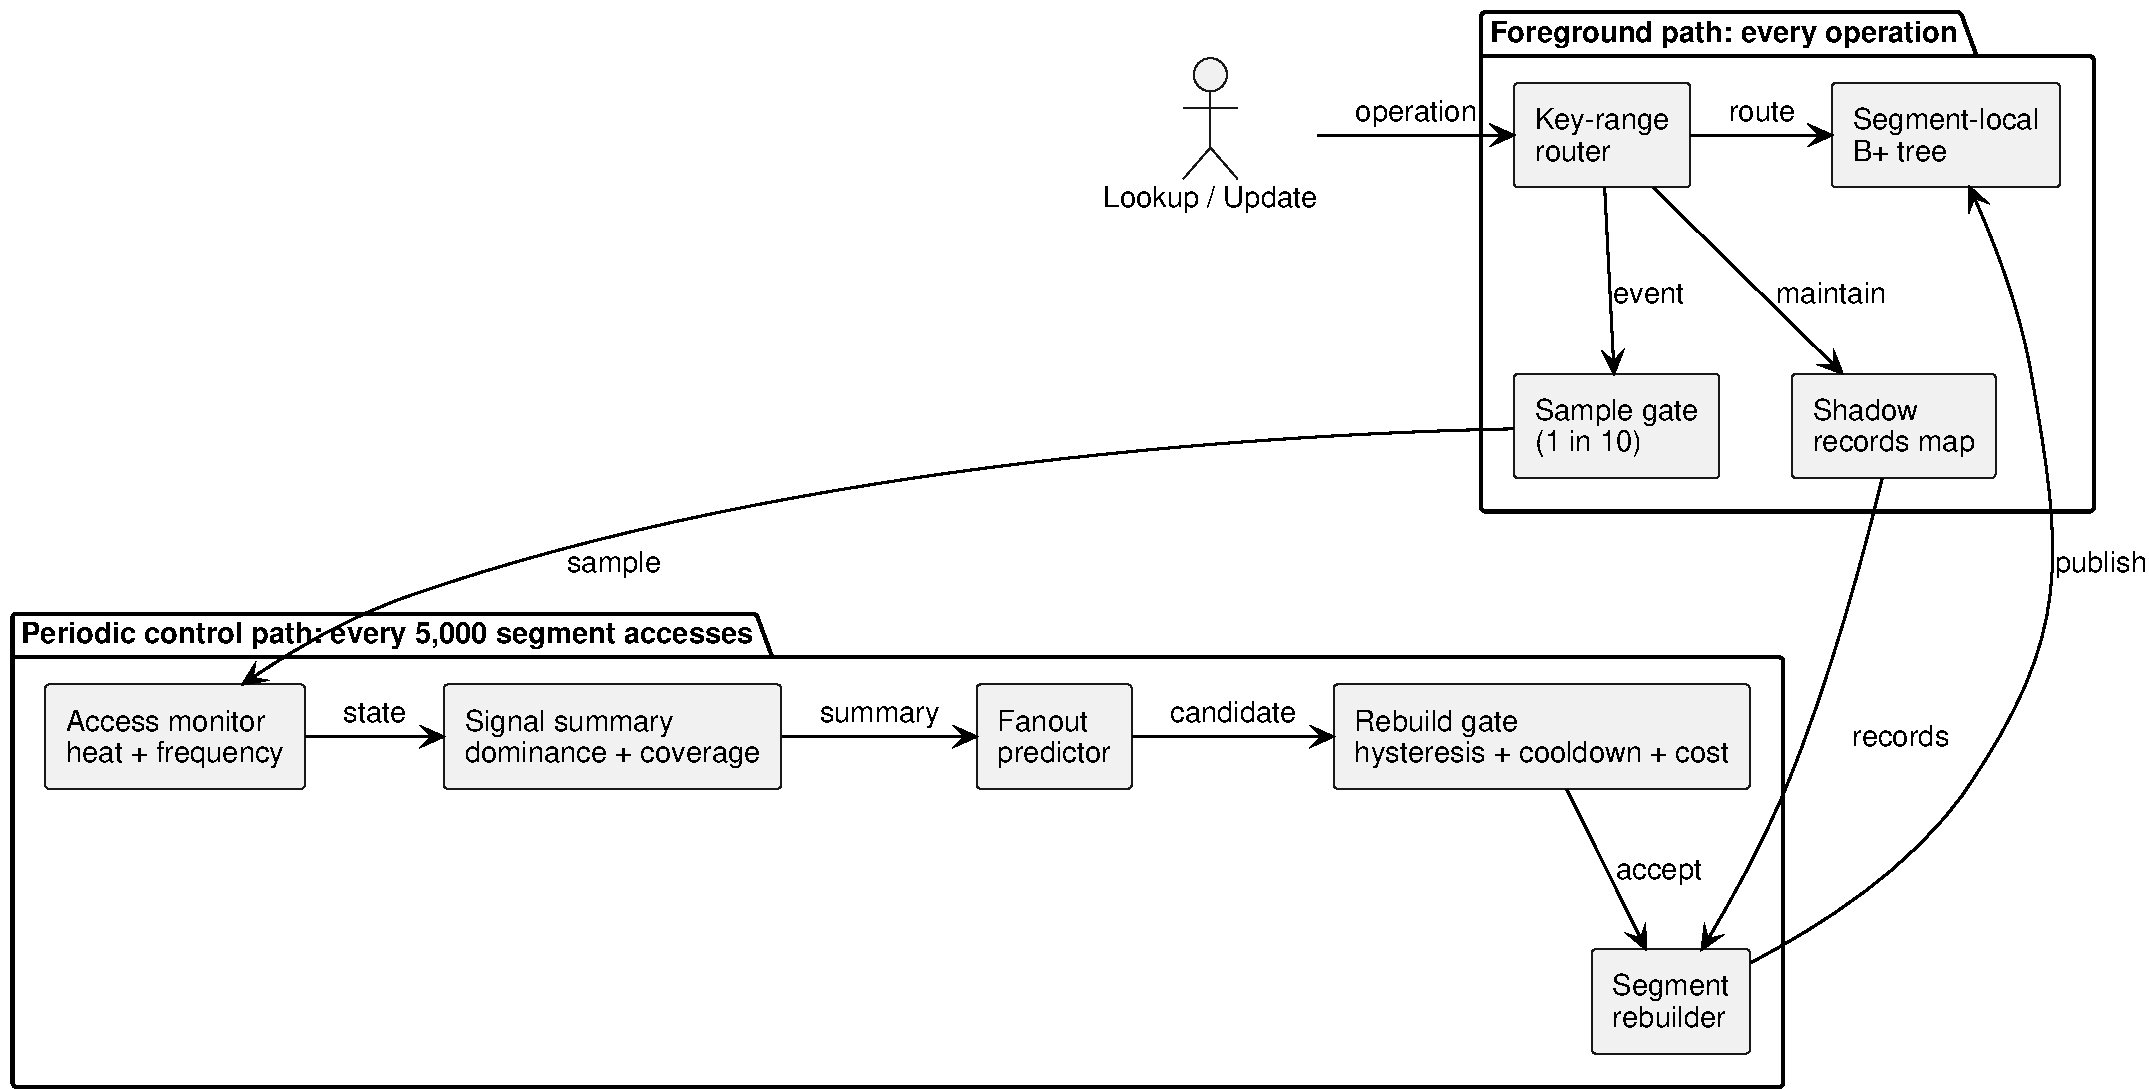
\includegraphics[width=\textwidth]{figures/fig_system_architecture.pdf}
  \caption{Architecture of Adaptive V1.  Routing,
  shadow-record maintenance, and the sample gate are foreground work.  Every
  5,000 segment accesses, the periodic path may build and publish a replacement
  tree after prediction and cost checks.}
  \Description{PlantUML component diagram separating the per-operation key
  routing, segment tree, records map, and sampling path from the periodic
  monitoring, prediction, rebuild gate, and segment reconstruction path.}
  \label{fig:architecture}
\end{figure*}

The separation matters experimentally.  A cost gate can eliminate an
unprofitable rebuild, but it cannot recover the routing, records-map, and
sampling work already paid while gathering evidence.  Conversely, disabling
adaptation while retaining those structures measures the recurring cost that
any policy in this implementation family must overcome.  This observation
motivates the component ladder in Section~\ref{sec:methodology}.

\subsection{Adaptive V2}

Adaptive V2 is a separate implementation variant designed directly from the
V1 ablation, not merely a different predictor.  It makes three structural
changes.  First, the B+ tree is the sole record store: inserts and updates do
not duplicate values in a shadow hash map, and lookups never fall back to such
a map.  Second, each segment uses a fixed-size frequency sketch with four rows
of 256 counters and a bounded 16-entry heavy-key candidate set.  A configurable
sample rate (16, 32, or 64 in the selected-regime experiment) limits foreground
monitoring work, so monitor memory is independent of the number of distinct
keys.  Third, once hysteresis, cooldown, and the cost gate accept a change, V2
exports the quiescent segment in key order and constructs the replacement
bottom-up with a sorted bulk loader.

V2 retains V1's eight-range router, candidate fanouts, and conservative control
logic so that the comparison isolates representation and observation costs.
The current V2 segment-replacement path is single-threaded: export, bulk load,
and root replacement occur at a quiescent benchmark point.  Consequently, the
multi-threaded scalability experiment evaluates only the static B+ tree and is
not evidence for concurrent V2 replacement.

\subsection{Baseline B+ Tree}

Our baseline is a C++11 B+ tree with configurable fanout, supporting insert,
update, point lookup, deletion, and range queries.  The baseline is deliberately
simple enough to isolate fanout effects, yet complete enough to preserve
standard B+ tree invariants.  The default static configuration uses fanout 64;
additional static baselines use fanouts 8, 16, 32, 128, and 256.

\subsection{Concurrency Boundary for Preloaded Trees}

The supported concurrent mode preloads all keys and keeps topology immutable.
Lookups traverse immutable internal nodes and synchronize with existing-value
updates at the target leaf.  A ThreadSanitizer diagnostic found a genuine race
in the separate structural-insert path, so we do not claim concurrent insert,
split, merge, deletion, or adaptive replacement.  These operations require
quiescence.  The supplementary material gives pseudocode and the exact safety
boundary; concurrency is ancillary to the single-threaded adaptation result.

\subsection{Monitoring}

The monitor tracks approximate heat for nodes or key ranges.  The segmented
tree records key identifiers, so the resulting summary describes access
concentration inside a segment rather than physical-node residency.  To limit
overhead, the outer segmented tree forwards one in ten accesses to the
monitor.  The monitor uses 64 metadata shards, sampled access counts, lazy
decay with factor 0.99, and an exponential moving average:
\[
  h_{t+1} = \alpha a_t + (1-\alpha)h_t.
\]
Here \(a_t=1\) for a sampled touch and \(\alpha=0.1\); decay is applied when a
tracked identifier is next inspected or touched.  The monitor exposes tracked
identifiers, decay, and aggregate statistics.  It is intentionally
lightweight, but it still increments a segment counter on every operation and
occasionally performs a hash-table lookup, timestamp read, lock acquisition,
and metadata update.  Its map also grows with the distinct sampled keys in the
finite benchmark run.  The ablation therefore reports both throughput and the
number of monitored identifiers instead of treating monitoring as free.

\subsection{Prediction Policies}

We implement three global policies.  A Q-learning policy maps coarse heat
states to actions that decrease, maintain, or increase fanout.  A regression
policy predicts fanout from heat and access count.  An ant-colony-inspired
policy maintains pheromone scores over heat/action pairs.  These policies are
included not because we expect them all to win, but to test whether the result
depends on policy choice.  In our measurements, policy sophistication is not
the main limiter; the common monitoring and metadata path is.

\subsection{Segmented Adaptation}

The most important adaptive design is segmented.  It partitions the key space
into fixed ranges.  Each segment owns its own B+ tree, monitor, records map,
and adaptation state.  Segment-level rebuilds are less disruptive than global
rebuilds and match shifting hot-region workloads better.  The segmented design
also enables clean ablations because we can disable records, monitoring, and
adaptation independently.

For a key domain \([K_{\min},K_{\max}]\) and \(S\) segments, routing uses
integer arithmetic to compute
\[
  s(k)=\min\!\left(S-1,
    \left\lfloor\frac{(k-K_{\min})S}
    {K_{\max}-K_{\min}+1}\right\rfloor\right).
\]
This is \(O(1)\), but it adds bounds checks, an indirection through the segment
array, and a second ownership boundary before every tree operation.  More
importantly, the \texttt{records} map is not a few bytes of policy metadata:
it is a complete key/value image of the segment.  Maintaining it duplicates
logical records and adds a hash-table update on writes.  We retain this design
because it makes reconstruction explicit and safe in the single-threaded
adaptive experiments; Section~\ref{sec:discussion} discusses alternatives.

\subsection{Cost-Aware Rebuild Gate}

The adaptive tree does not rebuild merely because a predictor recommends a new
fanout.  A cost-aware gate rejects rebuilds when the expected benefit is too
small, when evidence is weak, or when a segment is inside a cooldown period.
This gate reduces unnecessary rebuilds, but it does not remove ongoing access
path costs.

Algorithm~\ref{alg:rebuild-gate} gives the exact decision flow used by the
segmented tree.  The policy first summarizes the sampled monitor state, then
requires directional stability through repeated votes.  A segment is rebuilt
only if the cooldown has expired and the estimated benefit exceeds estimated
rebuild cost.  This is deliberately conservative: rejected rebuilds are
counted and reported as cost skips in the experiments.

The concrete gate requires at least 20 samples.  A fanout jump of at least
\(4\times\) needs two consistent votes; a smaller change needs three.  After a
rebuild, a segment cannot rebuild again for four adaptation intervals, or
20,000 segment accesses in the reported configuration.  Shrinking additionally
requires heat of at least 0.68 and either an 8\% dominant-key fraction or a
15\% hot-key fraction.  Growing requires the segment to have started below
fanout 64, heat at most 0.35, at least 16 tracked keys, and a dominant-key
fraction below 2\%.  These thresholds deliberately bias the system toward
\emph{not} rebuilding; they reduce catastrophic oscillation while exposing
the recurring cost of gathering enough evidence to reject a change.

\begin{algorithm}[t]
\caption{Cost-aware fanout rebuild gate}
\label{alg:rebuild-gate}
\begin{algorithmic}[1]
\Require Segment $s$, sampled monitor state, current fanout $f$
\Ensure Either rebuild to $f'$ or defer adaptation
\State $H \gets$ aggregate heat score of sampled keys in $s$
\State $D \gets$ dominant access fraction in $s$
\State $U \gets$ number of sampled unique keys/nodes
\State $f_p \gets \textsc{PredictFanout}(H,D,U)$
\State $f' \gets \textsc{ClampToPolicyBands}(f_p,H,D)$
\If{$f'=f$}
  \State count maintained fanout; defer next check
  \State \Return
\EndIf
\If{$f'$ changes direction relative to pending vote}
  \State reset pending target to $f'$ with one vote
\Else
  \State increment vote count for $f'$
\EndIf
\If{votes for $f'$ are below hysteresis threshold}
  \State count hysteresis skip; defer next check
  \State \Return
\EndIf
\If{segment is inside rebuild cooldown}
  \State count cooldown skip; defer until cooldown expires
  \State \Return
\EndIf
\State $B \gets \textsc{EstimateBenefit}(s,f,f',H,D,U)$
\State $C \gets \textsc{EstimateRebuildCost}(s)$
\If{$B \le C$}
  \State count cost skip; defer next check
  \State \Return
\EndIf
\State rebuild segment records into a new B+ tree with fanout $f'$
\State publish rebuilt segment; reset pending votes
\end{algorithmic}
\end{algorithm}

\paragraph{Rebuild complexity.}
V1 constructs an empty B+ tree at fanout \(f'\) and inserts every entry from
the segment's shadow records map.  For \(n_s\) records this costs
\(O(n_s\log_{f'}n_s)\) comparisons and allocations under ordinary insertion.
V2 instead exports the segment's leaves in sorted order and builds leaf and
internal levels bottom-up in \(O(n_s)\) time and space.  This removes repeated
searches and reduces allocation count, but it does not make a fanout change
constant time: export and construction still copy the complete segment.  The
gate uses a conservative linear rebuild score for V2 and an
\(n_s(1+\log_2 n_s)\) score for V1; both are engineering heuristics rather than
calibrated nanosecond predictors.  Their purpose is to reject clearly
unprofitable changes and report the rejection reason.

\section{Experimental Methodology}
\label{sec:methodology}

\subsection{Implementation and Platform}

The prototype is implemented in C++11.  The local experiments are compiled
with GCC 6.3.0 under Windows/MinGW on an ASUS laptop.  The codebase contains
roughly 2700 lines across the baseline
tree, monitor, predictor, adaptive policies, segmented tree, tests, and
benchmarks.  These local experiments run on one Windows 11 machine with a 12th-generation
Intel Core i5-12500H (12 physical cores, 16 hardware threads) and 16~GiB of
RAM.  The GPU is not used.  This machine is intentionally modest: the goal is
to study main-memory index overhead, not to rely on a large server or an
accelerator.

Table~\ref{tab:parameters-main} lists the principal settings.  The stationary
experiments use 100K records so all variants fit comfortably in memory; the
thread and sliding-hotspot experiments use one million records to exercise a
larger index while remaining practical on the same machine.  Unless noted,
the initial fanout is 64, the key domain is divided into eight equal ranges,
and adaptation is considered every 5,000 accesses to a segment.

\begin{table}[t]
\centering
\caption{Principal experimental parameters.}
\label{tab:parameters-main}
\resizebox{\columnwidth}{!}{%
\begin{tabular}{ll}
\toprule
Parameter & Setting \\
\midrule
Local compiler / platform & GCC 6.3.0 / Windows 11 \\
Local machine & ASUS i5-12500H, 16 threads, 16 GiB \\
Selected campaign & Kaggle Xeon, 4 vCPU, GCC 11.4.0 \\
Scale campaign & Kaggle Xeon, 4 vCPU, GCC 11.4.0 \\
Phase-length campaign & Kaggle EPYC 7B12, 4 vCPU, GCC 13.3.0 \\
Default / candidate fanouts & 64 / 8--256 \\
Segments / sampling & 8 / V1: 1/10; V2: 1/16--1/64 \\
Adaptation interval & 5,000 accesses \\
YCSB records / operations & 100K / 100K \\
YCSB Zipf parameter & 0.99 \\
Shifting operations / phase & 30K \\
Repeated trials & 5 \\
Thread records / operations & 1M / 10M \\
Sliding windows & $5\times1$M operations \\
Scale records / operations & 100K--5M / 1M \\
Phase study records / operations & 1M / 10M \\
Phase lengths & 10K, 100K, 1M, 5M, 10M \\
\bottomrule
\end{tabular}
}
\end{table}

\subsection{Compared Indexes and Oracles}

The baseline family contains a monolithic static B+ tree at fanout 64 and 256,
plus a static regional index with eight independently allocated trees.  The
shifting experiment sweeps regional fanout over
\(\{8,16,32,64,128,256\}\).  The adaptive family contains global RL,
regression, and ant-colony-inspired policies; a segmented tree with adaptation
disabled; Adaptive V1 with growing monitoring and shadow records; and Adaptive
V2 with bounded monitoring, no shadow map, and sorted bulk loading.  These are
not claimed as state-of-the-art learned-index competitors.  They test whether
changing both policy sophistication and implementation cost alters the dominant
cost conclusion within one common B+ tree implementation.

The phase oracle is a diagnostic upper bound.  It knows the next phase boundary
and hot segment, rebuilds that segment at fanout 8, 16, or 32, and reports both
operation-only throughput and throughput including measured reconfiguration
time.  A second retrospective envelope chooses the best measured static
regional fanout for each phase.  The oracle answers RQ1: if advance knowledge
cannot beat a static baseline, an online detector has no opportunity to
capture.  It is not presented as an implementable competitor.

The artifact additionally implements \emph{Perfect-V1} and \emph{Perfect-V2}.
They receive the selected fanout and phase boundary from a measured
phase-oracle file but still pay their variant's real reconstruction cost.  The
completed campaign contains 300 Perfect rows: three regimes, five seeds, ten
repetitions, and two implementations.  These rows separate prediction error
from actuation cost; the retrospective zero-cost oracle remains the deliberately
optimistic opportunity bound.

\subsection{Workloads}

We evaluate six workload families.

\textbf{YCSB-style workloads.}  Workload A is 50\% reads and 50\% updates,
workload B is 95\% reads and 5\% updates, and workload C is read-only.  Keys
follow a Zipfian distribution with \(\theta=0.99\), matching the skewed access
pattern used in many storage-system studies \cite{cooper2010benchmarking}.

\textbf{Shifting hot regions.}  Four phases target segment 0, segment 7, the
full key domain uniformly, and segment 3.  Each phase contains 30K operations.
This workload favors adaptation because the profitable regional fanout can
change over time, and the oracle receives the phase boundary and hot segment.

\textbf{Wikipedia pageview trace.}  We replay 30K operations on each of ten
consecutive days of a trace built from top Wikipedia articles using
Wikimedia's pageview data \cite{wikimediaPageviews}.  The trace is highly
skewed and supplies a real popularity distribution, although it is not a full
database transaction trace.

\textbf{Overhead ablation.}  We run a seven-row ladder: Static B+Tree, Static
Region, Static Region + Monitor, Segmented No Records, Segmented Records Only,
Segmented Monitor + Records, and Segmented Full Adaptive.  The ladder isolates
routing, shadow-record maintenance, monitoring, and adaptive decision/rebuild
costs without assuming every adjacent difference is statistically separable.

\textbf{Concurrent workload.}  A preloaded one-million-key tree
executes ten million operations with 95\% reads and 5\% in-place updates at 1,
4, 8, 16, and 32 worker threads.  The revised implementation restricts this
workload to immutable topology and leaf-synchronized point reads and
existing-value updates; fresh performance measurements are pending.  It does
not evaluate concurrent structural mutation or segment replacement.

\textbf{Sliding hotspot.}  Five one-million-operation windows each direct
80\% of accesses to a disjoint 20\% range of a one-million-key domain.  The
operation mix is 95\% reads and 5\% updates.  This tests whether the control
loop safely reacts when old evidence becomes stale at every window boundary.

\textbf{Scale sensitivity.}  A separate stationary-Zipf campaign compares
Static fanout 64 with Adaptive V2 at 100K, 1M, and 5M records.  At each scale,
five seeds and ten repetitions yield 50 exact seed/repetition pairs.  Each run
uses one million measured operations, a 95/5 read/update mix, sample rate 1/32,
and the same eight-segment V2 implementation and six fanout candidates.

\textbf{Phase-length break-even.}  A separate shifting-workload campaign
holds the database at one million records and each run at ten million measured
operations while varying phase length over 10K, 100K, 1M, 5M, and 10M.
For each of five seeds, six Static-Regional fanouts provide a measured
phase-aware zero-cost schedule.  Five repetitions of Static-Regional,
Perfect-V2, and Adaptive-V2 then form 125 exact trios.  The resulting 150
oracle-grid and 375 paid-decomposition runs use 95\% reads, 5\% updates,
Zipf 0.99, hot fraction 0.05, and sample rate 1/32.

\subsection{Measurement and Statistical Treatment}

For each workload, the operation sequence is generated once from a fixed seed
and replayed across all index variants.  Index construction is timed
separately and excluded from operation throughput.  Throughput is total
completed operations divided by wall-clock run time.  YCSB records every
operation latency; the larger sliding-hotspot benchmark samples one latency
per 1,024 operations to bound instrumentation cost.  A checksum and miss count
prevent dead-code elimination and detect semantic disagreement.

YCSB, shifting-hot-region, and overhead-ablation experiments are each repeated
five times.  We report arithmetic means, sample standard deviations, and
two-sided 95\% confidence intervals using Student's \(t\) distribution with
four degrees of freedom.  The thread, initial sliding-hotspot, and ten-day
Wikipedia experiments are descriptive single campaigns and are not assigned
trial-to-trial confidence intervals.  We therefore emphasize large,
cross-workload effects and disclose high-variance cases instead of treating
small ordering differences as significant.

We additionally run a selected-regime validation on a four-vCPU Kaggle CPU
instance using GCC 11.4.0, one million records, and one million measured
operations per run.  The campaign contains 1,740 completed runs and no failed
or partial runs.  Adaptive/static comparisons match seed and repetition; 95\%
hierarchical bootstrap intervals resample the five workload seeds and then the
ten repetitions within each seed.  Oracle comparisons match each seed to its
static calibration.  Because this campaign uses a different machine, we report
within-machine ratios and do not pool absolute throughput across hosts.
The local YCSB, shifting, Wikipedia, ablation, concurrency, and sliding-hotspot
results therefore refer to the ASUS i5-12500H/Windows platform; the broad and
selected-regime campaigns, including Perfect, refer to the Kaggle Xeon/Linux
platform and GCC 11.4.0.  The scale campaign also uses that Kaggle
Xeon/Linux toolchain, but is analyzed as a separate 300-run cohort identified
by machine fingerprint \texttt{f410f7064c081e00}; absolute throughput is not
pooled with earlier campaigns.
The phase-length campaign is a third isolated Kaggle cohort on an AMD EPYC
7B12 host with GCC 13.3.0 and machine fingerprint
\texttt{f0521629f96fce19}.  Its 125 trios use hierarchical paired-bootstrap
intervals over seeds and repetitions; absolute throughput is again not pooled
across machines.

\section{Results}

\subsection{Stationary YCSB}

Figure~\ref{fig:ycsb} and Table~\ref{tab:ycsb} show the YCSB results.
Segmented adaptation loses on all three workloads.  On YCSB-A it reaches
\(0.81\times\) of static fanout 64.  On YCSB-B it reaches \(0.74\times\);
on YCSB-C it reaches \(0.67\times\).  Static fanout 256 wins YCSB-B by
roughly \(6\%\), showing that fanout choice matters, but the adaptive path is
too costly to capture this gain.

The uncertainty supports the same conclusion with one caveat.  On YCSB-A,
static fanout 64 is 4.70M\(\pm\)0.36M operations/s and segmented adaptation is
3.83M\(\pm\)0.36M; their 95\% intervals are separated.  On YCSB-C the
intervals are also separated (7.04M\(\pm\)0.52M versus
4.74M\(\pm\)0.41M).  Fanout-64 YCSB-B is noisy, with a 19.9\% coefficient of
variation, so its interval overlaps the adaptive result.  The stronger static
fanout-256 comparison is 6.68M\(\pm\)0.57M versus
4.65M\(\pm\)0.46M, whose intervals do not overlap.  We therefore do not claim
that every static ordering is significant; we claim that the best static
configuration is consistently faster than online segmentation.

Policy choice does not rescue the global design.  Across YCSB-A/B/C, the
ant-colony-inspired tree reaches only 0.43/0.34/0.33 of fanout-64 throughput,
regression reaches 0.28/0.23/0.21, and RL reaches 0.20/0.16/0.16.  The
segmented policy is substantially better because it localizes rebuilds, yet it
still loses.  This ordering points away from prediction accuracy as the sole
problem: all global variants share expensive whole-tree adaptation, while the
best adaptive variant still pays the common foreground path.

\begin{figure}[t]
  \centering
  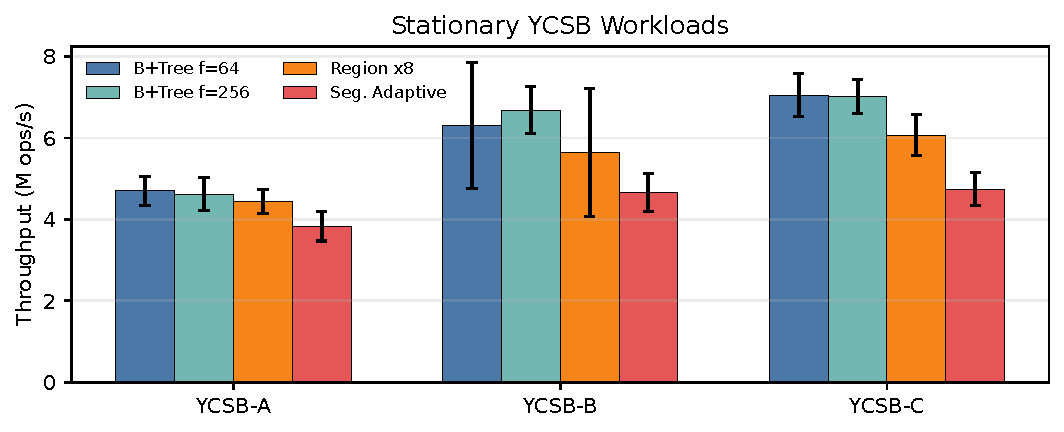
\includegraphics[width=\linewidth]{figures/fig_ycsb_throughput.pdf}
  \caption{Five-trial YCSB throughput.  Error bars show 95\% confidence
  intervals.  Segmented adaptation is consistently below static fanout 64.}
  \Description{Bar chart comparing throughput for static and adaptive indexes
  on YCSB workloads A, B, and C.}
  \label{fig:ycsb}
\end{figure}

\begin{table}[t]
\centering
\caption{Five-trial YCSB throughput summary.}
\label{tab:ycsb}
\begin{tabular}{lrrrr}
\toprule
Workload & Static f64 & Best static & Seg. adaptive & Seg./f64 \\
\midrule
YCSB-A & 4.70M & 4.70M & 3.83M & 0.81 \\
YCSB-B & 6.30M & 6.68M & 4.65M & 0.74 \\
YCSB-C & 7.04M & 7.04M & 4.74M & 0.67 \\
\bottomrule
\end{tabular}
\end{table}

\subsection{Shifting Hot Regions}

The shifting workload gives adaptation a fairer opportunity because locality
changes over time.  Figure~\ref{fig:shifting} plots selected per-phase
results.  The oracle with hot fanout 32 reaches \(1.08\times\) aggregate
throughput over static fanout 64, confirming that fanout adaptation has
headroom.  However, segmented adaptation reaches only \(0.92\times\).  Static
regional fanout 256 reaches \(1.13\times\), showing that coarse static
partitioning can be more effective than online adaptation.

The phase breakdown also warns against selecting a single favorable phase.
Static regional fanout 256 reaches \(1.35\times\) fanout 64 in Hot-S7 but only
\(0.93\times\) in Hot-S0.  Oracle-hot fanout 32 ranges from
\(0.98\times\) to \(1.18\times\) across measured phases.  Thus locality does
change the preferred layout, satisfying the premise of adaptation, but the
phase samples are variable: several static rows have coefficients of variation
above 20\%.  We use the five-trial aggregate and the oracle/static envelopes
as directional evidence rather than claiming a universally optimal regional
fanout.

\begin{figure}[t]
  \centering
  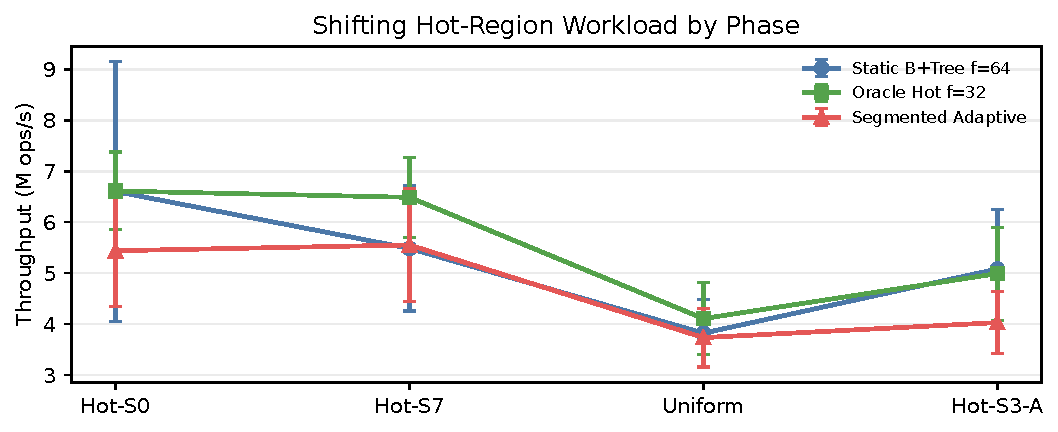
\includegraphics[width=\linewidth]{figures/fig_shifting_phases.pdf}
  \caption{Shifting hot-region throughput by phase.  The oracle shows
  measurable headroom, but online segmented adaptation does not capture it.}
  \Description{Line chart of throughput across hot-region phases for static,
  oracle, and segmented adaptive indexes.}
  \label{fig:shifting}
\end{figure}

\begin{table}[t]
\centering
\caption{Aggregate shifting workload throughput.}
\label{tab:shifting}
\begin{tabular}{lrr}
\toprule
Index & Throughput & vs f64 \\
\midrule
Static Region f256 & 5.53M & 1.13 \\
Oracle Hot f32 & 5.29M & 1.08 \\
Static B+Tree f256 & 5.24M & 1.07 \\
Static B+Tree f64 & 4.86M & 1.00 \\
Segmented Adaptive & 4.49M & 0.92 \\
\bottomrule
\end{tabular}
\end{table}

\subsection{Wikipedia Pageview Trace}

Table~\ref{tab:wiki} shows the real-trace result.  Static fanout 256 and
fanout 64 are nearly identical: 10.42M and 10.39M operations/s.  Thus the
workload has almost no fanout-selection headroom at this scale.  Segmented
adaptation reaches 8.40M operations/s, or \(0.81\times\) of static fanout 64.
The trace is skewed, but the hot working set is small enough that static
fanout choice is not the limiting factor.

The ten daily runs make the absence of headroom visible in another way.
Fanout-64 daily throughput ranges from roughly 9.18M to 11.20M operations/s,
whereas fanout-256 ranges from 10.01M to 10.75M.  Their aggregate means differ
by only about 0.3\%, smaller than the variation across days.  The adaptive
tree nevertheless performs 37 policy evaluations and one rebuild over the
trace.  Extreme popularity skew therefore does not imply a useful fanout
signal: once the active set is already cache-resident, extra heat tracking can
remain pure overhead.

\begin{table}[t]
\centering
\caption{Wikipedia pageview trace throughput.}
\label{tab:wiki}
\begin{tabular}{lrr}
\toprule
Index & Throughput & vs f64 \\
\midrule
Static B+Tree f256 & 10.42M & 1.00 \\
Static B+Tree f64 & 10.39M & 1.00 \\
Static Region f32 & 10.19M & 0.98 \\
Static Region x8 & 9.88M & 0.95 \\
Segmented No Adapt & 8.79M & 0.85 \\
Segmented Adaptive & 8.40M & 0.81 \\
\bottomrule
\end{tabular}
\end{table}

\subsection{Clean Overhead Ablation}

Figure~\ref{fig:overhead} and Table~\ref{tab:overhead} isolate the access-path
costs.  The values are intentionally not monotone in every row: cache
placement, routing, and run-to-run noise can make one row faster than the
previous row.  The robust pattern is that the full adaptive path is below
static on Zipf-A and Zipf-B and below the best static regional rows.  In
Zipf-A, the records-only row reaches 4.90M operations/s, the monitor-plus-
records row reaches 4.60M operations/s, and full adaptation reaches 3.91M
operations/s.

Repeated trials make two conclusions defensible.  First, individual adjacent
rows are not always ordered: for example, records-only is faster than the
no-records row on Zipf-B.  We treat such inversions as cache placement and
run-order noise, not as negative-cost metadata.  Second, the end-to-end gaps
are much larger.  On Zipf-A, the lower endpoint for Static B+Tree is 4.57M
operations/s, while the upper endpoint for Full Adaptive is 4.21M.  On Zipf-B
the corresponding endpoints are 6.52M and 6.10M.  Uniform-B intervals overlap,
so we make no significance claim there.  The controlled conclusion for RQ3 is
that monitoring and decisions are first-order costs under skew, while no
single neighboring row should be over-interpreted.

\begin{figure}[t]
  \centering
  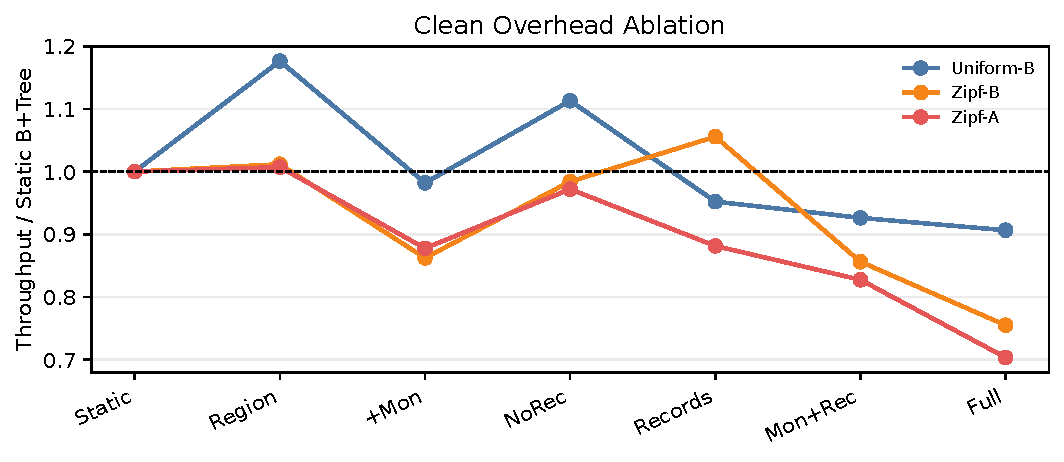
\includegraphics[width=\linewidth]{figures/fig_overhead_ablation.pdf}
  \caption{Clean overhead ablation normalized to Static B+Tree.  The full
  adaptive path includes routing, records, monitoring, policy checks, and
  rebuild decisions.}
  \Description{Line chart of normalized throughput across the seven ablation
  configurations.}
  \label{fig:overhead}
\end{figure}

\begin{table*}[t]
\centering
\caption{Clean overhead ablation.  Ratios are relative to the previous
conceptual baseline named in each column.}
\label{tab:overhead}
\resizebox{\textwidth}{!}{%
\begin{tabular}{lrrrrrrr}
\toprule
Workload & Region/Static & Monitor/Region & NoRec/Region & Rec/NoRec &
MonRec/Rec & Full/MonRec & Full throughput \\
\midrule
Uniform-B & 1.18 & 0.83 & 0.95 & 0.86 & 0.97 & 0.98 & 4.79M \(\pm\) 0.41M \\
Zipf-A & 1.01 & 0.87 & 0.97 & 0.91 & 0.94 & 0.85 & 3.91M \(\pm\) 0.30M \\
Zipf-B & 1.01 & 0.85 & 0.97 & 1.07 & 0.81 & 0.88 & 5.68M \(\pm\) 0.42M \\
\bottomrule
\end{tabular}}
\end{table*}

\subsection{Concurrent Validation Boundary}

The concurrency experiment is restricted to a tree preloaded before workers
start.  Workers issue point lookups and updates of existing values; they do not
insert new keys or trigger splits, merges, deletion, or replacement.  A
ThreadSanitizer diagnostic found a genuine race in an earlier structural
insert test: an optimistic reader examined ordinary internal-node fields while
a writer modified them.  The subsequent version check did not make that access
legal under the C++ memory model.

The revised supported path traverses immutable internal nodes and acquires the
target leaf lock before reading keys or values.  Existing-value updates use the
same lock.  Deterministic validation checks the exact final state, key count,
checksum, lookups, ranges, structural invariants, and unexpected misses for
read-only, update-only, and mixed workloads.  We do not report the earlier
thread-throughput measurements because they used the superseded optimistic
value-read path.  Fresh scalability measurements require a clean TSan result
for the revised path and are outside the evidence reported here.

\subsection{Rapidly Shifting Hotspots}

We also add a sliding-hotspot benchmark.  The workload contains one million
keys and five one-million-operation windows.  In each window, 80\% of accesses
target a Zipfian hot region covering 20\% of the key space; the hot region
moves to a disjoint range in the next window.  This benchmark is intentionally
hostile to stale predictors.  Figure~\ref{fig:dynamic} and
Table~\ref{tab:dynamic} show that the adaptive tree does not catch up: the
cost gate evaluates many adaptation opportunities but performs no rebuilds,
and the full segmented adaptive path reaches only \(0.63\times\) the static
B+ tree throughput.  This strengthens the paper's negative result because the
workload gives adaptation fresh skew but too little safe headroom to exploit.

The rejection counters reveal why.  Across the five windows, the policy runs
264 adaptation evaluations, rejects 247 at the cost gate, and performs zero
rebuilds.  Hence the controller is not losing because it repeatedly rebuilds
the wrong segment.  It is losing while correctly deciding that available
evidence does not justify reconstruction.  The first adaptive window reaches
3.44M operations/s, but later windows fall to 2.22--2.89M as monitored state
accumulates; fanout remains 64 throughout.  This is a particularly strong
negative case for fine-grained control: conservative actuation avoids rebuild
spikes, yet observation and shadow-state maintenance still consume 37\% of
the static baseline's throughput.

\begin{figure}[t]
  \centering
  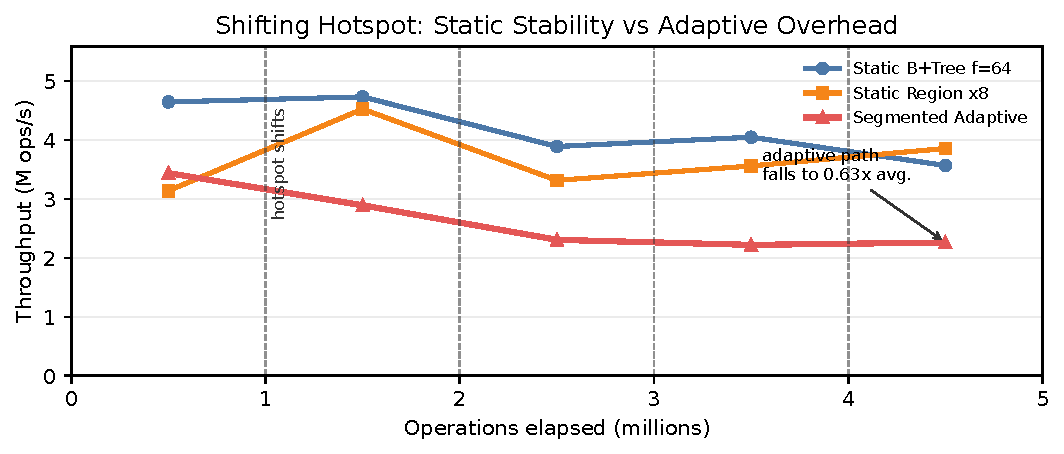
\includegraphics[width=\linewidth]{figures/fig_dynamic_hotspot.pdf}
  \caption{Sliding-hotspot throughput by one-million-operation window.  The
  adaptive tree tracks accesses but remains below static fanout 64.}
  \Description{Line chart comparing static, static regional, and segmented
  adaptive throughput over five shifting-hotspot windows.}
  \label{fig:dynamic}
\end{figure}

\begin{table}[t]
\centering
\caption{Sliding-hotspot aggregate throughput.}
\label{tab:dynamic}
\begin{tabular}{lrr}
\toprule
Index & Throughput & vs Static f64 \\
\midrule
Static B+Tree f64 & 4.18M & 1.00 \\
Static Region x8 & 3.68M & 0.88 \\
Segmented Adaptive & 2.62M & 0.63 \\
\bottomrule
\end{tabular}
\end{table}

\subsection{Selected-Regime Validation}

The preceding sliding-hotspot experiment establishes the failure mode, but a
single trajectory cannot determine whether the result is stable across
sampling rates and workload seeds.  We therefore use a measured static-fanout
screening campaign to select three regimes: a long, highly skewed regime with
little expected headroom (Zero); a long regime near the selection boundary
(Borderline); and a rapidly changing regime with the largest measured
headroom (High).  For each regime we evaluate Adaptive V1 and the cost-aware
Adaptive V2 at sample rates 16, 32, and 64.  Each cohort contains five seeds
and ten repetitions per seed.  Separate static-fanout calibration runs
construct a retrospective, zero-cost phase oracle on the same machine and
binary.

Figure~\ref{fig:selected-validation} and
Table~\ref{tab:selected-validation} report seed/repetition-matched ratios.
The best V2 setting is sample rate 64 in all three regimes.  Nevertheless,
V2 reaches only \(0.881\times\), \(0.890\times\), and \(0.931\times\) of
static regional throughput.  Every 95\% interval lies below one.  The
zero-cost oracle confirms genuine but narrow opportunity:
\(1.032\times\), \(1.029\times\), and \(1.041\times\), respectively.
Thus the conclusion is not that fanout never matters; it is that this online
mechanism cannot capture a benefit of this size cheaply enough.

\begin{figure}[t]
  \centering
  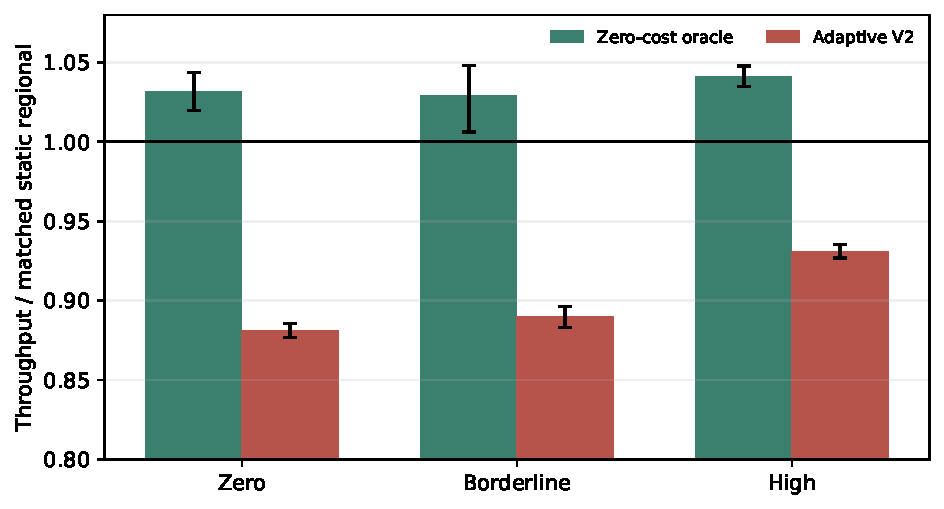
\includegraphics[width=\linewidth]{figures/fig_dynamic_selected_validation.pdf}
  \caption{Selected-regime validation with paired 95\% bootstrap intervals.
  A retrospective zero-cost oracle is above static, while Adaptive V2 is
  significantly below its matched static-regional baseline in every regime.}
  \Description{Grouped bars compare zero-cost oracle and Adaptive V2
  throughput ratios in zero, borderline, and high-headroom regimes.}
  \label{fig:selected-validation}
\end{figure}

\begin{table}[t]
  \centering
  \caption{Selected-regime validation.  Adaptive columns use 50 paired runs;
  oracle ratios use five matched seeds.}
  \label{tab:selected-validation}
  \resizebox{\columnwidth}{!}{\begin{tabular}{lrrrr}
\toprule
Regime & Oracle/static & Adapt./static & 95\% CI & Penalty ($\mu$s/op) \\
\midrule
Zero & 1.032 & 0.881 & [0.877, 0.886] & 0.0211 \\
Borderline & 1.029 & 0.890 & [0.883, 0.896] & 0.0219 \\
High & 1.041 & 0.931 & [0.927, 0.936] & 0.0199 \\
\bottomrule
\end{tabular}
}
\end{table}

The time-domain comparison in Figure~\ref{fig:selected-costs} makes the
break-even failure explicit.  Across the three regimes, the oracle saves
0.0049, 0.0050, and 0.0106~\us/op, whereas V2 adds 0.0211, 0.0219, and
0.0199~\us/op relative to its paired static baseline.  Even in the High
regime, ongoing adaptive cost is about \(1.9\times\) the maximum retrospective
benefit before charging any uncertainty or prediction error.  Longer phases
cannot repair the first two regimes because their recurring cost already
exceeds their per-operation benefit.

\begin{figure}[t]
  \centering
  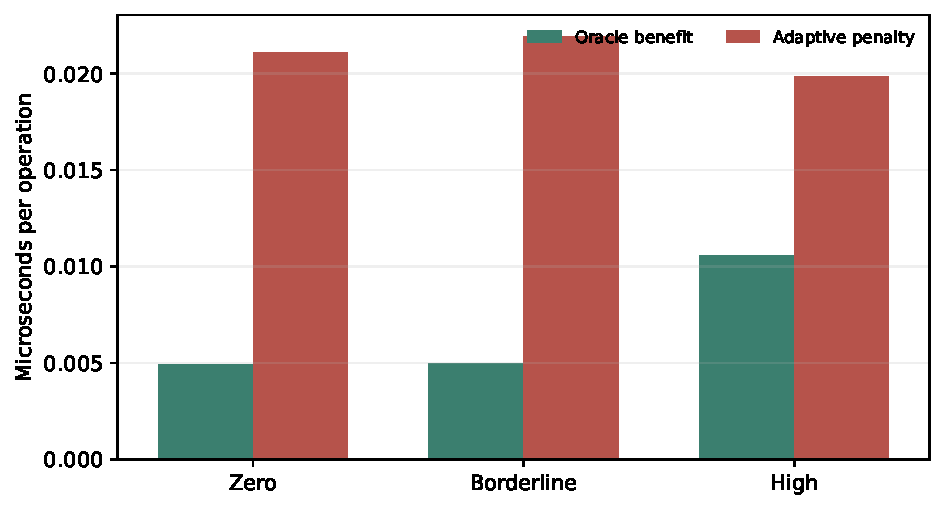
\includegraphics[width=\linewidth]{figures/fig_dynamic_selected_costs.pdf}
  \caption{Oracle benefit and Adaptive V2 penalty in time per operation.  The
  online penalty exceeds the available fanout benefit in every regime.}
  \Description{Grouped bars compare oracle time savings with adaptive time
  penalties for three selected workload regimes.}
  \label{fig:selected-costs}
\end{figure}

\subsection{Perfect Detection and Actuation Cost}

Perfect prediction does not imply profitable adaptation.  We pair each
Perfect execution with STATIC-REGIONAL, Adaptive V1, and Adaptive V2 using the
same seed, repetition, workload fingerprint, checksum, and zero miss count.
The zero-cost oracle is measured once per seed at repetition zero; its fanout
schedule is reused for the ten deterministic repetitions, so it is
workload-paired but is not treated as 50 independent oracle measurements.
Table~\ref{tab:perfect-decomposition} reports hierarchical bootstrap intervals.

\begin{table*}[t]
  \centering
  \caption{Perfect-detector decomposition at sample rate 32.  Ratios are to
  matched STATIC-REGIONAL.  Rebuild share is measured rebuild-routine time
  divided by total wall time and is a lower bound on full actuation overhead.}
  \label{tab:perfect-decomposition}
  \resizebox{\textwidth}{!}{\begin{tabular}{llrrr}
\toprule
Regime & Variant & Mean vs. static & 95\% CI & Rebuild share \\
\midrule
Zero & Oracle zero-cost & 1.030 & [1.018, 1.041] & -- \\
Zero & PERFECT-V1 & 0.127 & [0.126, 0.129] & 83.5\% \\
Zero & PERFECT-V2 & 0.490 & [0.484, 0.497] & 38.0\% \\
Zero & ADAPT-V1 & 0.500 & [0.495, 0.507] & 30.1\% \\
Zero & ADAPT-V2 & 0.879 & [0.867, 0.890] & 0.0\% \\
\midrule
Borderline & Oracle zero-cost & 1.021 & [1.001, 1.043] & -- \\
Borderline & PERFECT-V1 & 0.223 & [0.221, 0.226] & 71.6\% \\
Borderline & PERFECT-V2 & 0.625 & [0.619, 0.633] & 25.2\% \\
Borderline & ADAPT-V1 & 0.531 & [0.526, 0.538] & 15.0\% \\
Borderline & ADAPT-V2 & 0.885 & [0.878, 0.892] & 0.0\% \\
\midrule
High & Oracle zero-cost & 1.044 & [1.039, 1.049] & -- \\
High & PERFECT-V1 & 0.006 & [0.006, 0.007] & 98.5\% \\
High & PERFECT-V2 & 0.064 & [0.059, 0.071] & 77.0\% \\
High & ADAPT-V1 & 0.797 & [0.794, 0.799] & 0.0\% \\
High & ADAPT-V2 & 0.923 & [0.916, 0.929] & 0.0\% \\
\bottomrule
\end{tabular}
}
\end{table*}

In the Zero and Borderline regimes, Perfect-V2 reaches only \(0.490\times\)
and \(0.625\times\) static, despite oracle opportunities of \(1.030\times\)
and \(1.021\times\).  In the High regime, the 10K-operation phase length
creates 100 phase boundaries.  The oracle schedule changes fanout often enough
to trigger 470.4 segment rebuilds per run on average.  Perfect-V1 consequently
reaches \(0.006\times\) static and spends 98.5\% of wall time inside measured
rebuild routines; Perfect-V2 reaches \(0.064\times\) and spends 77.0\%.  The
extreme ratios are not checksum failures or denominator artifacts: rebuilds
are charged inside the same wall-clock interval as operations, and observed
counts exactly equal oracle fanout transitions times eight segments.

The online-control difference has the opposite sign from a naive predictor
story.  Adaptive V2 is faster than Perfect-V2 in all three regimes because its
cost gate rejects most or all changes.  Thus the decomposition attributes the
dominant loss to actuation, while also showing that conservative online control
can be beneficial precisely by refusing an oracle-selected layout whose
short-lived operation-only advantage cannot repay reconstruction.

\subsection{Scale Sensitivity}

Figure~\ref{fig:adaptive-scale} and Table~\ref{tab:adaptive-scale} report 150
exact Static-f64/Adaptive-V2 pairs across three database sizes.  Adaptive V2
moves toward parity as the database grows: its paired throughput ratio is
\(0.848\times\) at 100K records, \(0.888\times\) at 1M, and \(0.926\times\)
at 5M.  The corresponding 95\% hierarchical paired-bootstrap intervals are
[0.839, 0.857], [0.877, 0.900], and [0.912, 0.940].  All remain below one, so
V2 is significantly slower than Static f64 throughout the tested 100K--5M
range, although the mean penalty narrows from approximately 15.2\% to 7.4\%.

\begin{figure}[t]
  \centering
  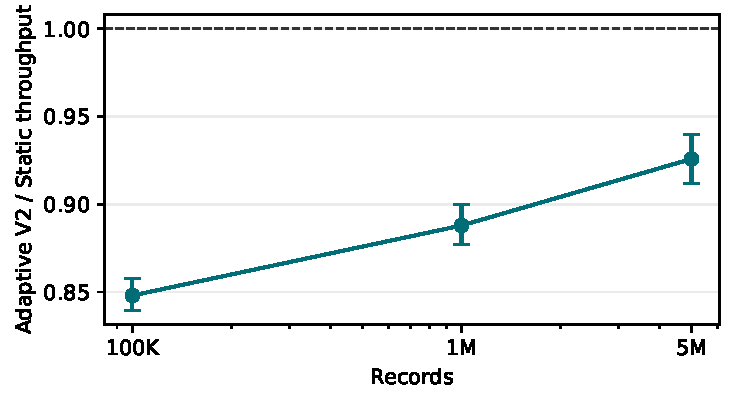
\includegraphics[width=\linewidth]{figures/adaptive_scale.pdf}
  \caption{Adaptive V2 throughput normalized to its exact paired Static-f64
  run.  Error bars are 95\% hierarchical paired-bootstrap intervals; the
  dashed line denotes parity.  The gap narrows with scale but remains
  statistically below parity through 5M records.}
  \Description{A three-point line plot rises from 0.848 at 100K records to
  0.926 at 5M records.  All confidence intervals lie below the parity line.}
  \label{fig:adaptive-scale}
\end{figure}

\begin{table}[t]
  \centering
  \caption{Adaptive V2 scale sensitivity.  Each row summarizes 50 exact
  seed/repetition pairs; intervals are 95\% hierarchical paired-bootstrap
  confidence intervals for the throughput ratio.}
  \label{tab:adaptive-scale}
  \small
  \begin{tabular}{rrrrr}
    \toprule
    Records & Static & Adaptive V2 & V2/Static & Rebuilds \\
            & (Mops/s) & (Mops/s) & (95\% CI) & (mean) \\
    \midrule
    100K & 5.85 & 4.96 & 0.848 [0.839, 0.857] & 1.0 \\
    1M   & 3.39 & 3.00 & 0.888 [0.877, 0.900] & 0.0 \\
    5M   & 2.45 & 2.27 & 0.926 [0.912, 0.940] & 0.0 \\
    \bottomrule
  \end{tabular}
\end{table}


Adaptive V2 performs one rebuild per run on average at 100K and zero rebuilds
at both 1M and 5M.  Consequently, the residual large-scale penalty cannot be
attributed to restructuring in those two cohorts; it is the recurring cost of
monitoring, segment routing, and controller execution.  This agrees with the
break-even model: increasing scale makes adaptation more competitive as fixed
work is better amortized, but eliminating rebuild cost does not eliminate the
online term \(\mu\).  Historical static-oracle sweeps show 4.3--5.8\% mean
headroom across these sizes, but those measurements use a different source
fingerprint and repetition structure.  We therefore report them only as
unpaired context, not as exact comparisons to this scale cohort.  These data
establish persistence, not asymptotic behavior: they do not determine whether
V2 could reach parity beyond 5M records or on another platform or workload.

We also repeat the same three-scale comparison on the independent ASUS
i5-12500H/Windows platform using five seeds and three repetitions (45 exact
pairs).  Mean V2/static ratios are \(0.949\times\), \(0.925\times\), and
\(0.990\times\) at 100K, 1M, and 5M records.  The paired 95\% intervals are
[0.909, 1.033], [0.896, 0.967], and [0.932, 1.119], respectively.  Thus the
1M replication independently confirms a significant loss, while 100K and 5M
are inconclusive rather than wins.  Absolute rates are not pooled across the
Windows laptop and Kaggle Xeon cohorts.

\subsection{Phase Length and Break-Even}

We next hold the database and measured work fixed at 1M records and 10M
operations while varying phase length from 10K to 10M operations.  For each
of five seeds, a six-fanout regional sweep constructs a measured phase-aware
zero-cost oracle.  Five repetitions of Static-Regional, Perfect-V2, and
Adaptive-V2 then form 125 exact trios.  All trios match on workload
fingerprint and checksum and report zero misses.  Figure~\ref{fig:phase-length-v2}
and Table~\ref{tab:phase-length-v2} report hierarchical paired-bootstrap
intervals; the measured oracle schedule is treated as one seed-level
observation rather than five independent repetitions.
This campaign ran separately on a Kaggle AMD EPYC 7B12 host; we normalize
only within exact trios and do not pool its absolute throughput with the
earlier Kaggle Xeon or Windows cohorts.

\begin{figure}[t]
  \centering
  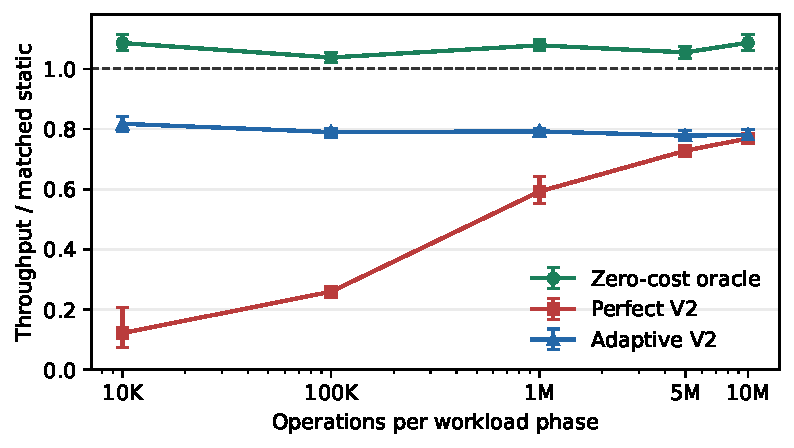
\includegraphics[width=\linewidth]{figures/phase_length_v2.pdf}
  \caption{Phase-length decomposition.  The zero-cost oracle exposes layout
  opportunity at every tested phase length.  Paid Perfect V2 improves as
  rebuilds become less frequent, but neither Perfect V2 nor Adaptive V2
  reaches static parity through the tested 10M-operation phase.}
  \Description{A line plot over phase lengths from ten thousand to ten
  million operations.  The zero-cost oracle remains above parity.  Perfect
  V2 rises from 0.122 to 0.769, while Adaptive V2 remains near 0.8.}
  \label{fig:phase-length-v2}
\end{figure}

\begin{table*}[t]
  \centering
  \caption{Phase-length decomposition at 1M records and 10M operations.
  Ratios use exact matched Static-Regional runs; intervals are 95\%
  hierarchical paired-bootstrap CIs.}
  \label{tab:phase-length-v2}
  \small
  \begin{tabular}{rrrrrr}
    \toprule
    Phase & Oracle/Static & Perfect-V2/Static & Adaptive-V2/Static &
    Perfect rebuilds & Adaptive rebuilds \\
    \midrule
    10K  & 1.086 [1.060, 1.113] & 0.122 [0.075, 0.205] & 0.818 [0.792, 0.842] & 2344.0 & 0 \\
    100K & 1.038 [1.020, 1.055] & 0.259 [0.240, 0.277] & 0.790 [0.779, 0.802] & 473.6  & 0 \\
    1M   & 1.078 [1.060, 1.096] & 0.593 [0.553, 0.641] & 0.792 [0.783, 0.802] & 54.4   & 0 \\
    5M   & 1.055 [1.034, 1.074] & 0.728 [0.716, 0.744] & 0.778 [0.764, 0.796] & 9.6    & 0 \\
    10M  & 1.087 [1.060, 1.115] & 0.769 [0.755, 0.785] & 0.781 [0.765, 0.797] & 8.0    & 0 \\
    \bottomrule
  \end{tabular}
\end{table*}


The oracle ratios range from \(1.038\times\) to \(1.087\times\), and every
oracle interval excludes parity.  Thus all five cohorts contain genuine
fanout opportunity.  Perfect V2, which is given the measured target schedule
but pays for physical replacement, rises from \(0.122\times\) at 10K to
\(0.769\times\) at 10M as its mean rebuild count falls from 2,344 to eight.
It nevertheless remains significantly below static at every tested length.
This separates an operation-only layout advantage from the cost of realizing
that layout.

Adaptive V2 performs zero rebuilds in all five cohorts and remains between
\(0.778\times\) and \(0.818\times\) static.  Its controller therefore protects
against the catastrophic short-phase actuation cost, but recurring monitoring,
routing, and decision work still prevents parity.  At 10M, the mean
Perfect-minus-Adaptive difference is \(-0.012\) and its 95\% interval
[-0.025, 0.001] includes zero: paid perfect detection has caught up with, but
does not significantly exceed, conservative online control.  We observe no
paid-actuation or online break-even within 10K--10M operations per phase.  We
do not extrapolate this finite range to longer phases, other workloads, or
other machines.

\subsection{Cross-Workload Synthesis}

Table~\ref{tab:synthesis} answers RQ1 and RQ2 in one view.  The opportunity
column is the best measured static configuration for stationary workloads and
the phase-aware oracle for the shifting workload, normalized to static fanout
64.  It is deliberately generous to the adaptive hypothesis.  YCSB-A,
YCSB-C, and Wikipedia expose essentially no selection headroom; online
adaptation cannot win there unless it is free.  YCSB-B and shifting do expose
6--8\% headroom, but segmented adaptation gives up 26\% and 8\% relative to
fanout 64.  The selected-regime campaign independently reproduces the same
pattern: even its High regime offers only 4.1\% oracle headroom while Adaptive
V2 gives up 6.9\%.  The headroom is real, but smaller than the cost of finding
and acting on it.

\begin{table*}[t]
\centering
\caption{Opportunity versus achieved segmented-adaptive throughput.  Values
are normalized to static fanout 64.}
\label{tab:synthesis}
\begin{tabular}{lrrrl}
\toprule
Workload & Opportunity & Seg. adaptive & Gap to opportunity & Interpretation \\
\midrule
YCSB-A & 1.00 & 0.81 & $-0.19$ & No static headroom; recurring cost dominates \\
YCSB-B & 1.06 & 0.74 & $-0.32$ & Headroom exists but is not captured \\
YCSB-C & 1.00 & 0.67 & $-0.33$ & Read-only path magnifies overhead \\
Shifting hot regions & 1.08 & 0.92 & $-0.16$ & Oracle wins; online control still loses \\
Wikipedia trace & 1.00 & 0.81 & $-0.19$ & Skew without useful fanout separation \\
Sliding hotspot & --- & 0.63 & --- & Gate rejects all rebuilds, but tracking remains \\
Selected high-headroom & 1.041 & 0.931 & $-0.110$ & Paired CI excludes parity \\
\bottomrule
\end{tabular}
\end{table*}

The table also separates two kinds of negative result.  In a
\emph{no-opportunity} workload, the right response is an early bypass that
turns monitoring off.  In an \emph{uncaptured-opportunity} workload, the
research problem is to reduce observation and reconstruction cost below the
measured oracle gap.  A policy paper that reports only final throughput would
conflate these cases; oracle and ablation rows make the diagnosis actionable.

\subsection{Memory Reclamation and Reader Safety}

The supported concurrent mode avoids reclamation by construction.  It preloads
the tree before workers start, keeps topology immutable, performs only lookups
and existing-value updates, and destroys the tree only after workers join.
Leaf readers and value writers synchronize on the same version lock.  This
restricted mode does not support concurrent insertion, splitting, merging,
deletion, or node reclamation.

Segment rebuilds for adaptive fanout are more subtle.  In the current
experiments, segmented rebuilds are evaluated in the single-threaded adaptive
benchmarks, not concurrently with the multi-threaded lookup benchmark.  A
concurrent adaptive tree would need to retire replaced segment roots using
epoch-based reclamation: each worker publishes its active epoch before
traversal, writers place old roots on a retire list, and a retired tree is
freed only after all active readers have advanced beyond the retire epoch.
This is an engineering constraint rather than a change to the break-even
model; epoch management would add another small term to the online overhead
\(\mu\).

\section{Theoretical Analysis}

We now formalize the cost argument.  The theory has two roles.  First, it
shows that restructuring itself can be amortized if the algorithm waits for
enough evidence.  Second, it shows why that amortization is insufficient when
per-operation monitoring and metadata costs exceed the fanout benefit.

\subsection{Amortized Restructuring}

Let a segment maintain a nonnegative potential \(\Phi_t\).  Each operation
adds at most a constant \(\gamma\) units of potential.  A rebuild of cost
\(R_t\) is allowed only when \(\Phi_t \ge R_t\), and when it rebuilds the
algorithm spends \(R_t\) units of potential.

\begin{theorem}
If the rebuild rule above is enforced, restructuring has \(O(1)\) amortized
cost per operation.
\end{theorem}

\begin{proof}
Let \(a_t\) be the actual restructuring cost at operation \(t\), and define
the amortized cost
\[
  \hat{a}_t = a_t + \Phi_{t+1}-\Phi_t .
\]
If no rebuild occurs, \(a_t=0\) and \(\Phi_{t+1}-\Phi_t\le\gamma\), so
\(\hat{a}_t\le\gamma\).  If a rebuild occurs, then \(a_t=R_t\) and the
potential decreases by at least \(R_t\), except for the current operation's
new credit:
\[
  \Phi_{t+1}-\Phi_t \le \gamma - R_t .
\]
Thus \(\hat{a}_t \le R_t+\gamma-R_t=\gamma\).  Summing over \(T\)
operations telescopes the potential terms, giving total restructuring cost
\(O(T)\), or \(O(1)\) amortized cost per operation.
\end{proof}

\subsection{A Conditional Online Bound}

A multiplicative competitive claim requires assumptions about exploration;
otherwise an arbitrarily bad candidate fanout can make a testing epoch
arbitrarily expensive.  We therefore state the finite-candidate bound with
those assumptions explicit.  Consider a stable phase \(P\) of \(T_P\)
operations and candidate set \(\mathcal F\) of size \(k\).  Let \(c_P^\star\)
be the oracle operation cost in the phase.  The online policy spends at most
\(q\) operations testing each candidate, all tested candidates cost at most
\(\beta c_P^\star\), and its selected candidate costs at most
\(\alpha c_P^\star\).  Let \(\mu\) be recurring online overhead and \(R_P\)
the total restructuring cost in the phase.

\begin{theorem}
Under the conditions above, the phase cost of the online policy satisfies
\[
 \frac{\mathrm{Cost}_P(\mathrm A)}
      {\mathrm{Cost}_P(\mathrm{OPT})}
 \le
 \alpha
 + \frac{kq(\beta-\alpha)}{T_P}
 + \frac{\mu}{c_P^\star}
 + \frac{R_P}{T_Pc_P^\star}.
\]
\end{theorem}

\begin{proof}
At most \(kq\) operations are exploratory and cost at most
\(\beta c_P^\star\) each.  The remaining \(T_P-kq\) operations use the
selected candidate at cost at most \(\alpha c_P^\star\).  Adding recurring
and restructuring costs gives
\[
 \mathrm{Cost}_P(\mathrm A)
 \le kq\beta c_P^\star
 +(T_P-kq)\alpha c_P^\star+T_P\mu+R_P.
\]
Dividing by \(T_Pc_P^\star=\mathrm{Cost}_P(\mathrm{OPT})\) yields the
claim.
\end{proof}

For a double-exponential theoretical ladder, \(k=O(\log\log n)\).  The
implementation instead uses the constant candidate set
\[
  \mathcal F=\{8,16,32,64,128,256\}.
\]
With fixed \(q\), the exploration and rebuild
terms shrink in a long stable phase.  The recurring ratio
\(\mu/c_P^\star\) does not.  This is the formal reason that ``wait longer''
cannot repair the implementation when monitoring and shadow-state work already
exceed the oracle benefit.

\subsection{Break-Even Condition}

The measurements can be explained by a simple condition.  Consider a phase of
\(T\) operations in a segment with incumbent fanout \(F_0\) and candidate
fanout \(F_1\).  Let
\[
  \Delta = C(F_0,N_s)-C(F_1,N_s)
\]
be the per-operation fanout benefit.  Let \(m\), \(\rho\), and \(d\) be the
per-operation costs of monitoring, records metadata, and policy evaluation,
and let \(R\) be the one-time rebuild cost.  Adaptation improves total time
only if
\[
  T(\Delta - m - \rho - d) > R.
\]
Equivalently, if \(\Delta \le m+\rho+d\), no phase length can make online
adaptation profitable.

\begin{theorem}[Oracle-headroom lower bound]
Let \(B_{\max}\) be the per-operation improvement of a zero-overhead oracle
over an incumbent layout.  Any online policy that retains the same incumbent
and pays recurring overhead \(\mu\), nonnegative policy regret \(E\), and
nonnegative amortized restructuring cost \(R/T\) cannot outperform the
incumbent when \(B_{\max}\le\mu\).
\end{theorem}

\begin{proof}
Relative to the incumbent, the online policy's best possible net improvement
per operation is at most
\(B_{\max}-\mu-E-R/T\).  Because \(E\ge0\) and \(R/T\ge0\), this quantity is
nonpositive whenever \(B_{\max}\le\mu\).
\end{proof}

For multiple phases, the same accounting yields a regret decomposition.  If
phase \(i\) has length \(T_i\), oracle fanout \(f_i^\star\), selected fanout
\(g_i\), recurring overhead \(\mu_i\), and rebuild cost \(R_i\), then
\[
 \mathrm{Regret}=
 \sum_i T_i\!\left(c_{g_i}-c_{f_i^\star}\right)
 +\sum_i T_i\mu_i+\sum_i R_i.
\]
The first term is decision error; the latter two remain even under perfect
prediction.  Our oracle measures the maximum amount available to pay all three
terms, while the clean ablation estimates the recurring component.

The scale experiment sharpens this decomposition.  At 1M and 5M records,
\(R/T=0\) because V2 performs no rebuilds, yet its paired throughput remains
\(0.888\times\) and \(0.926\times\) static.  Thus scale narrows the observed
gap within the tested range, but the recurring term \(\mu\) remains large
enough to prevent break-even even when measured restructuring cost vanishes.

This model does not say that adaptation is impossible.  It says adaptation must
be judged at the same time scale as the operation it improves.  For in-memory
B-trees with sub-microsecond lookups, software monitoring and rebuild decisions
are expensive.  For disk-resident trees, remote memory, or very long stable
phases, the benefit term \(\Delta\) may become large enough to dominate.

\section{Discussion}
\label{sec:discussion}

\subsection{Interpretation}

Failure across multiple policies and cost-aware gates points to a cost/benefit
mismatch rather than one poor controller: the oracles expose useful fanout
choices, while the ablations show that observing and acting on them consumes
the opportunity.  The break-even condition nevertheless leaves room for
adaptation when I/O or remote-memory costs enlarge \(\Delta\), phases are long,
monitoring is hardware-assisted, or decisions operate at index or partition
granularity.

\subsection{Practical and Design Implications}

For in-memory indexes at this scale, static tuning and coarse regional layout
are safer.  Systems should first perform an \emph{opportunity test} over a few
offline layouts and enable coarse, phase-driven tuning only when the measured
gap pays for the controller.  V2 removes shadow records, bounds monitoring, and
bulk-loads replacements, yet reaches only \(0.881\)--\(0.931\times\) static
throughput in selected regimes.  Oracle baselines and component ablations are
therefore necessary to distinguish opportunity from realizable gain.

\subsection{Threats to Validity}

\textbf{Platform and scale.}  Local experiments use Windows on an ASUS laptop
with an Intel i5-12500H.  The selected and scale campaigns use a four-vCPU
Kaggle Xeon host with GCC 11.4.0; the phase-length campaign uses a separate
four-vCPU Kaggle EPYC host with GCC 13.3.0.  We compare variants only within a
machine and cohort.  Different cache sizes, NUMA placement, allocators, or
storage media can change both static fanout ordering and the relative cost of
metadata.  The scale campaign extends the tested range to 5M in-memory integer
keys, but does not establish asymptotic behavior or make a claim about
billion-key or disk-resident indexes.  The smaller cross-platform replication
contains only 15 pairs per scale; its wider intervals cross parity at 100K and
5M.

\textbf{Causal mechanism.}  We attribute costs to software components through
controlled configuration ablations and elapsed time.  The node-footprint
analysis motivates cache sensitivity but is not presented as direct evidence
of a particular microarchitectural event.

\textbf{Workload coverage and noise.}  Fixed seeds improve pairing but cover
one skew parameter and a bounded phase range.  Some five-trial shifting rows
have broad intervals, so we avoid claims from small adjacent differences.  The
Wikipedia trace supplies real popularity skew, but its point-operation replay
is not a complete database workload.

\textbf{Implementation boundary.}  This segmented design is not a lower bound
for all adaptive B-trees.  V2 still copies a complete segment and uses a
heuristic cost gate.  Concurrency validation covers only preloaded,
topology-immutable trees with synchronized lookups and existing-value updates;
structural mutation, adaptive replacement, and epoch reclamation are excluded.
Thus our claim is specific: for these implementations and in-memory workloads,
measured recurring cost consumes the available oracle headroom.

\section{Related Work}

B-trees are foundational ordered indexes
\cite{bayer1972organization,comer1979ubiquitous,graefe2011modern}.
Cache-conscious and cache-oblivious designs optimize layout, prefetching, and
memory transfers \cite{rao1999cache,rao2000making,chen2001fractal,bender2000cache},
while FAST, Masstree, HOT, and Wormhole explore architecture-sensitive
main-memory layouts \cite{kim2010fast,mao2012masstree,binna2018hot,wu2019wormhole}.
Concurrent and persistent trees instead optimize synchronization, indirection,
or recovery \cite{lehman1981efficient,graefe2010locking,sewall2011palm,
levandoski2013bw,oukid2016fptree,arulraj2018bztree}.  We isolate the runtime cost
of changing fanout online.

Workload-aware structures include splay trees, database cracking, adaptive
merging, ART, and learned indexes
\cite{sleator1985self,idreos2007database,idreos2011adaptive,leis2013adaptive,
kraska2018case,ding2020alex,galakatos2019fiting}.  Robustness studies show that
workload order and reorganization policy can dominate convergence
\cite{halim2012stochastic,schuhknecht2013uncracked}; dynamic learned indexes and
controlled benchmarks similarly motivate changing-distribution evaluation and
strong static baselines
\cite{ferragina2020pgm,kipf2020radixspline,tang2020xindex,wu2021lipp,
marcus2020benchmark}.  None isolates paid online fanout selection as we do.

Self-tuning systems select indexes, views, or configurations at coarser time
scales \cite{chaudhuri1998autoadmin,weikum2002selftuning,pavlo2017selfdriving,
vanaken2017automatic}.  Their amortization horizon reinforces our finding that
sub-microsecond access paths are a particularly harsh setting for adaptation.

\section{Conclusion}

Our experiments support a diagnostic negative result: measurable phase-aware
fanout headroom is consumed by monitoring, metadata, policy, and replacement.
The 1,740-run selected-regime campaign keeps every paired interval for the best
cost-aware configuration below static parity.  Across 100K--5M records, V2
narrows from \(0.848\times\) to \(0.926\times\), but remains slower even with
zero rebuilds at 1M and 5M.  Across 10K--10M-operation phases, zero-cost oracle
headroom is 3.8--8.7\%, yet paid Perfect V2 never reaches parity and
non-rebuilding Adaptive V2 retains recurring cost.

Adaptive-index evaluations should therefore report oracle opportunity and paid
overhead together.  Within our tested systems, platforms, and ranges,
fine-grained fanout adaptation does not replace static tuning or coarse regional
indexing.

\section*{Generative AI Disclosure}
Large language models were used to assist with code scaffolding and
boilerplate, and to improve the clarity, organization, and flow of the
manuscript.  The authors determined the research questions and system design,
conducted and validated the experiments, verified the mathematical analysis
and citations, interpreted the results, and take responsibility for the work.

\bibliographystyle{ACM-Reference-Format}
\bibliography{references}

\end{document}
